\documentclass[notes]{beamer}
\usepackage[latin1]{inputenc}
\usepackage{tikz}
\usetikzlibrary{arrows}
\usetikzlibrary{shapes.misc}
\usepackage{verbatim}
\usepackage{amsthm}
\usetheme{Warsaw}

\title{Homogeneity is Independent from Randomness}
\author{Li Ling Ko}
\institute{University of Notre Dame}
\date{22/29? January, 2018}
\setbeamertemplate{footline}[frame number]
\setbeamertemplate{theorems}[numbered]

\newcommand{\TODO}[1]{\textcolor{red}{TODO: #1}}
\newtheorem{thm}{Theorem}
\newtheorem*{thm*}{Theorem}
\newtheorem*{main-thm*}{Main Theorem}
\newtheorem{coro}{Corollary}
\newtheorem*{coro*}{Corollary}
\newtheorem{pf}{Proof}
\newtheorem*{pf*}{Proof}
\newtheorem{define}{Definition}
\newtheorem*{define*}{Definition}
\newtheorem{claim}{Claim}
\newtheorem*{claim*}{Claim}
\newtheorem*{fact*}{Fact}

\begin{document}
\begin{frame}
  \titlepage
\end{frame}

\begin{frame}{Notations}
  \begin{itemize}
    \item $\omega=\mathbb{N}$, $a,b,\ldots\in\omega$,
      $A,B,\ldots\subseteq\omega$, $\sigma,\tau\in\omega^{<\omega}$,
      $\mathcal{A},\mathcal{B},\ldots\subseteq\omega^\omega$.
    \item Trees $T$ are subsets of $\omega^{<\omega}$ closed under initial
      segments; i.e. $\sigma^{\frown}n\in T \rightarrow \sigma\in T$.
    \item Paths are functions $f:\omega\rightarrow\omega$. A tree contains
      a path $f$ iff $T$ contains every initial segment $f\restriction n$
      of $f$.
    \item $[T] :=\{f:f\; \text{is a path on}\; T\}$.
    \item Turing functionals on trees are partial-recursive functionals
      $\Gamma:2^{<\omega}\rightarrow\omega^{<\omega}$ where
      $\tau\in\Gamma^{\sigma^\frown n} \rightarrow
      \tau\in\Gamma^{\sigma}$. $\Gamma$ can be extended naturally to
      $\Gamma:2^\omega\rightarrow\omega^{\omega}$.
    \item Given set $A$ and cardinal $\kappa$, $[A]^\kappa
      :=\{B\subseteq A: |B|=\kappa\}$.
    \item Given $A\in[\omega]^\omega$, can think of $A$ as its characteristic
      function $c_A:\omega\rightarrow\{0,1\}$, or as their principal
      function $p_A:\omega\rightarrow\omega$ which is a strictly increasing
      function enumerating $A$.
  \end{itemize}
\end{frame}

\begin{frame}{Ramsey's Theorem ($\text{RT}$)}
  \begin{define*}[$c$-homogeneous]
    Given $k$-coloring $c:[\omega]^n\rightarrow k$, a subset
    $A\subseteq\omega$ is $c$-homogeneous if every $n$-tuple over $A$ is
    given the same color by $c$.
  \end{define*}

  \vspace{1em}
  \begin{define*}[Ramsey's Theorem]
    Fix $n,k\leq1$. $\text{RT}_k^n$ is the statement\\
    ``Every $k$-coloring $c:[\omega]^n\rightarrow k$ has an infinite
    $c$-homogeneous set.''\\
    RT is the statement $(\forall n)(\forall k)\; \text{RT}_k^n$.
  \end{define*}

  \vspace{1em}
  RT asserts homogeneity exists.
\end{frame}

\begin{frame}{Randomness}
  \begin{itemize}
    \item What is 1-random
    \item Lebesgue Measure
  \end{itemize}
\end{frame}

\begin{frame}{Strongly Omnisciently Computably Reducible
  ($\leq_{\text{soc}}$)}
  \begin{itemize}
    \item Define problem, solution
    \item Define $\leq_{\text{soc}}$ on WWKL, RT
    \item WWKL $\leq_{\text{soc}}$ WKL: From definition.
    \item WKL $\leq_{\text{soc}}$ KL: From definition.
  \end{itemize}
\end{frame}

\begin{frame}{KL $\leq_{\text{soc}}$ WKL}
  Given KL instance \textbf{P}, at each level, code branches into WKL
  instance \textbf{Q} using binary representation of branch number
\end{frame}

\begin{frame}{RT $\leq_{\text{soc}}$ WKL}
  \begin{itemize}
    \item Fix $k$-coloring $c:[\omega]^n\rightarrow k$.
    \item Define binary tree $T\subseteq 2^{<\omega}$ by
      \[\sigma\in T \Leftrightarrow \{n:\sigma(n)=1\}\; \text{is
      homogeneous}.\]
  \end{itemize}
\end{frame}

\begin{frame}{Homogeneity ``independent from'' Randomness}
  Dependencies under $\leq_{\text{soc}}$
  \vspace{2em}

  \begin{center}
    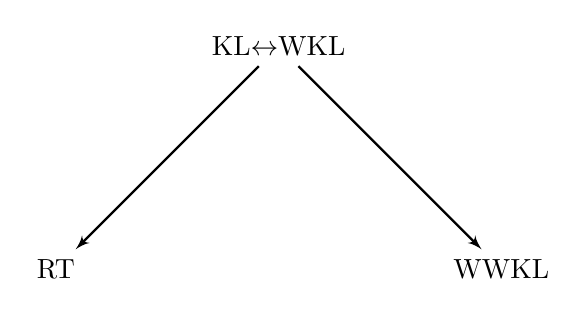
\begin{tikzpicture}[node distance=4cm,auto,thick,>=latex']
      \node (KL) {KL$\leftrightarrow$WKL};
      \node (WWKL) [below right of=KL] {WWKL};
      \node (RT) [below left of=KL] {RT};
      \draw[->] (KL) -- (RT);
      \draw[->] (KL) -- (WWKL);
      %\draw [->,red] (RT) -- coordinate (m) (WWKL);
      %\draw[shift={(m)},red](-0.1,-0.1)--(0.1,+0.1);
    \end{tikzpicture}
  \end{center}
\end{frame}

\begin{frame}{Bi-Hyperimmune sets}
  \begin{define}[Hyperimmune, Bi-hyperimmune]
    $A\subseteq\omega$ is \textbf{hyperimmune} if there is no effective way
    of knowing when new elements of $A$ have appeared.  Formally, no
    recursive function dominates $p_A$, the principal function of $A$. $A$
    is \textbf{bi-hyperimmune} if both $A$ and $\bar{A}$ are hyperimmune.
  \end{define}

  \begin{thm}
    Bi-hyperimmune sets exist.
  \end{thm}

  \textbf{Pf:} Enumerate recursive functions $f_0,f_1,\ldots$. At stage
  $s$, let $i$ be the number of elements in $A$ and $\bar{A}$ that has been
  defined so far. Put enough elements into $\bar{A}$ till the $(i+1)$-th
  element of $A$ exceeds that of $f_s$, then put the next element into $A$.
  This ensures that $f_s$ cannot tell when the $(i+1)$-th element of $A$
  has appeared. Repeat with roles of $A$ and $\bar{A}$ reversed.
  $\blacksquare$
\end{frame}

\begin{frame}{Class of sets computing subsets of hyperimmune is null}
  \begin{thm}
    \label{thm:bihyper-null}
    Given a hyperimmune set $A$, the class of sets that can compute an
    infinite subset of $A$ is null.
  \end{thm}

  \vspace{1em}
  \textbf{Proof idea:} Assume not. Then there are enough paths computing
  infinite subsets of $A$ such that we can effectively ask them to ``vote''
  for when new elements of $A$ must have appeared,
  $\Rightarrow\Leftarrow$.\\

  \vspace{1em}
  \textbf{Pf:} Fix Turing functional $\Phi$. Write $\mathcal{B} :=\{X:
  \Phi^X\in[A]^\omega\}$. Suffices to show $\mu(\mathcal{B})=0$. Assume
  $\mu(\mathcal{B})=4m>0$.
\end{frame}

\begin{frame}{Class of sets computing subsets of hyperimmune is null}
  \begin{itemize}
    \item Approximate $\mathcal{B}$ by open cover
      $\mathcal{O}\supseteq\mathcal{B}$ with
      $\mu(\mathcal{O}-\mathcal{B})<m$.
    \item Approximate $\mathcal{O}$ by basic open sets
      $[\sigma_0],\ldots,[\sigma_n] \subseteq\mathcal{O}$ with
      \[\mu(\mathcal{O}-([\sigma_0]\cup\ldots\cup[\sigma_n])) <m.\]
    \item Fix effective enumeration of branches $\sigma$ in
      $[\sigma_0]\cup\ldots\cup[\sigma_n]$.
    \item At stage $s=0$, wait till a measure of $2m$ of such $\sigma$'s
      finds an element via $\Phi$; let $f(0)$ be the largest element found.
    \item Since $[\sigma_0]\cup\ldots\cup[\sigma_n]$ approximate
      $\mathcal{B}$ tightly, such $\sigma$'s exist.
      \begin{align*}
        \mu(\text{``true'' voters})>2m,\\
        \mu(\text{``false'' voters})<2m.
      \end{align*}
      Thus $f(0)\geq p_A(0)$.
    \item At stage $s+1$, wait till a measure of $2m$ of $\sigma$'s
      finds an element $>f(s)$; let $f(s+1)$ be the largest
      element found. $\blacksquare$
  \end{itemize}
\end{frame}

\begin{frame}{$\text{RT}_2^1$ $\nleq_{\text{soc}}$ WWKL}
  \begin{thm}
    $\text{RT}_2^1$ $\nleq_{\text{soc}}$ WWKL.
  \end{thm}

  \vspace{1em}
  \textbf{Pf:} Let $c:\omega\rightarrow\{0,1\}$ be a 2-coloring of the
  graph of a fixed bi-hyperimmune $A$, that is,
  \[c(n)=0 \Leftrightarrow n\in A.\]
  
  From Theorem~\ref{thm:bihyper-null}, the class of sets computing an
  infinite subset of $A$ or of $\bar{A}$ is null, thus the class of
  $c$-homogeneous sets is null. Therefore given arbitrary tree
  $T\subseteq\omega^{<\omega}$ of positive measure, some path must fail to
  compute any $c$-homogeneous set. $\blacksquare$
\end{frame}

\begin{frame}{RT $\nleq_{\text{soc}}$ WKL, WKL $\nleq_{\text{soc}}$ WWKL}
  \begin{coro}
    \label{coro:rt-wwkl}
    RT $\nleq_{\text{soc}}$ WWKL.
  \end{coro}
  \textbf{Pf:} Follows from previous theorem. $\blacksquare$

  \vspace{2em}
  \begin{coro}
    WKL $\nleq_{\text{soc}}$ WWKL.
  \end{coro}
  \textbf{Pf:} Follows from transitivity of $\leq_\text{soc}$,
  RT $\leq_{soc}$ WKL, and RT $\nleq_{\text{soc}}$ WWKL. $\blacksquare$
\end{frame}

\begin{frame}{Recursive-Encodability, $\Pi_1^0$-Encodability}
  For the remaining directions
  \begin{itemize}
    \item WKL $\nleq_{\text{soc}}$ RT
    \item WWKL $\nleq_{\text{soc}}$ RT
  \end{itemize}

  we need the following definitions and characterizations:
  \vspace{1em}

  \begin{define}[Recursive-Encodable $A\subseteq\omega$]
    $A\subseteq\omega$ is recursively-encodable if given any
    $X\in[\omega]^\omega$, some subset of $X$ computes $A$.
  \end{define}

  \begin{define}[$\Pi_1^0$-encodable $\mathcal{A}\subseteq\omega^\omega$]
    $\mathcal{A}\subseteq \omega^{\omega}$ is $\Pi_1^0$-encodable if
    \TODO{write out definition}.
  \end{define}
\end{frame}

\begin{frame}{Characterizing Encodability}
  \newtheorem*{main-thm*}{Main Theorem}
  \begin{main-thm*}[Characterizing $\Pi_1^0$-encodable
  $\mathcal{A}\subseteq\omega^\omega$]
    $\mathcal{A}\subseteq \omega^{\omega}$ compact. Then
    \[\mathcal{A}\; \text{is}\; \Pi_1^0\text{-encodable}\; \Leftrightarrow
    \mathcal{A}\; \text{contains non-empty}\; \Sigma_1^1\; \text{subset}.\]
  \end{main-thm*}

  \begin{coro*}[Characterizing Recursively-Encodable $A\subseteq\omega$]
    $A\subseteq\omega$ recursively-encodable $\Leftrightarrow$ $A$ is
    hyperarithmetic.
  \end{coro*}

  \vspace{1em}
  From Main Theorem, suffices to show
  \begin{itemize}
    \item $A\subseteq\omega$ is hyperarithmetic $\Leftrightarrow$
      $\{A\}\subseteq\omega^\omega$ is $\Sigma_1^1$
    \item $A\subseteq\omega$ recursively-encodable $\Leftrightarrow$
      $\{A\}\subseteq\omega^\omega$ is $\Pi_1^0$-encodable
  \end{itemize}
\end{frame}

\begin{frame}{$A$ hyperarithmetic $\Leftrightarrow$ $\{A\}$ is $\Sigma_1^1$}
  \begin{align*}
    \;&A\subseteq\omega\; \text{hyperarithmetic}\\
    \Rightarrow\; & A\in\Sigma_1^1\\
    \Rightarrow\; & A=\{n:(\exists f)(\forall s)\; [R(f\restriction s,n)]\}\\
    \Rightarrow\; & \{A\}= \{g:(\exists f)(\forall s)(\forall n)\\
    &[R(f\restriction s,n) \rightarrow g(n)=1 \wedge \neg R(f\restriction s,n)
      \rightarrow g(n)=0]\}\\
    \Rightarrow\; &\{A\}\subseteq\omega^\omega\; \text{is}\; \Sigma_1^1,\\
    &\\
    \Rightarrow\; & \{A\}= \{g:(\exists f)(\forall s)\; [Q(f\restriction
      s,g\restriction s)]\}\\
    \Rightarrow\; &
      \begin{cases}
        A=\{n:(\exists g)(\exists f)(\forall s)\; [Q(f\restriction
          s,g\restriction s) \leftrightarrow g(n)=1]\}\\
        A=\{n:(\forall g)(\forall f)(\exists s)\; [\neg Q(f\restriction
          s,g\restriction s) \rightarrow g(n)=0]\}
      \end{cases}\\
    \Rightarrow\; &A\in\Delta_1^1\\
    \Leftrightarrow\; &A\subseteq\omega\; \text{hyperarithmetic}.\\
  \end{align*}
\end{frame}

\begin{frame}{$A$ recursively-encodable $\Leftrightarrow$
$\{A\}$ is $\Pi_1^0$-encodable}
  \begin{align*}
    \;&A\subseteq\omega\; \text{recursively-encodable}\\
    \Leftrightarrow\; & (\forall X\in[\omega]^\omega)(\exists Y\subseteq
      X)\; [Y\geq_T A]\\
    \Rightarrow\; & (\forall X\in[\omega]^\omega)(\exists Y\subseteq X)\;
      [\{A\}\supseteq \{Y\}]\\
    \Rightarrow\; &\{A\}\subseteq\omega^\omega\; \text{is}\;
      \Pi_1^0\text{-encodable},\\
    &\\
    \Rightarrow\; & (\forall X\in[\omega]^\omega)(\exists Y\subseteq
      X)(\exists T^Y,f^Y\leq_T Y)\\
    &[\{A\}=[T^Y]\; \wedge\; (\forall n)\; [\max_{\sigma\in
    T^Y\cap\omega^n}\{\sigma(n)\}<f(n)]]\\
    \Rightarrow\; & (\forall X\in[\omega]^\omega)(\exists Y\subseteq
      X)\; [Y\geq_T A]\\
    \Rightarrow\; &A\subseteq\omega\; \text{recursively-encodable}.\\
  \end{align*}
\end{frame}

\begin{frame}{$\Sigma_1^{1}$-immunity basis theorem (fixed machine)}
  \begin{lemma}[$\Sigma_1^{1}$-immunity basis, fixed machine]
    $\mathcal{A}$ compact, contains no $\Sigma_1^{1}$-set
    ($\neq\emptyset$). Fix $\Sigma_1^{1}$-predicate $P(X,Y)$,
    $\Sigma_1^{1}$-set $\mathcal{B}_0\neq\emptyset$. Then
    $\mathcal{B}_0$ has a $\Sigma_1^{1}$-subset
    $\mathcal{B}\neq\emptyset$ such that for every $X\in\mathcal{B}$,
    $\mathcal{A}$ does not contain the $\Sigma_1^{1,X}$-set
    $\{Y:P(X,Y)\}$ (if $\neq\emptyset$).
  \end{lemma}

  \vspace{1em}
  \textbf{Pf:} \underline{Case 1}: For every $X\in\mathcal{B}_0$,
  $\{Y:P(X,Y)\}\subseteq\mathcal{A}$. Then $\bigcup_{X\in\mathcal{B}_0}
  \{Y:P(X,Y)\}$ will be a $\Sigma_1^{1}$-subset of $\mathcal{A}$,
  $\Rightarrow\Leftarrow$.

  \vspace{1em}
  \underline{Case 2}: For some $X_0\in\mathcal{B}_0$, $\{Y:P(X_0,Y)\}$
  contains a path $Y_0$ outside $\mathcal{A}$. By compactness of
  $\mathcal{A}$, $Y_0$ has an initial segment $\sigma$ outside
  $\mathcal{A}$. This $\Sigma_1^{1}$-subset of $\mathcal{B}_0$ works:
  \[\mathcal{B}:= \{X\in\mathcal{B}_0: (\exists Y\succ\sigma)\; P(X,Y)\}.\;
  \blacksquare\]
\end{frame}

\begin{frame}{Gandy-Harrington topology is Baire}
  \begin{thm}[Gandy-Harrington]
    \label{thm:gandy-harrington}
    The topology on $\omega^\omega$ where open sets are generated by the
    $\Sigma_1^{1}$-sets is known as the Gandy-Harrington topology.  This
    topology is Baire, i.e. the countable union of dense open sets is
    dense.
  \end{thm}

  \vspace{1em}
  \textbf{Proof Idea:} Given dense open sets
  $\mathcal{D}_0,\mathcal{D}_1,\ldots$ and
  $\Sigma_1^1$-set $\mathcal{O}=\{f:(\exists g)\; R(f,g)\}$, iteratively
  construct $f\in\bigcap_{n\in\omega}\mathcal{D}_n$ and $g$ witnessing
  $f\in\mathcal{O}$:
  
  \vspace{1em}
  At stage $n$, $[f\restriction n]\cap\mathcal{O} \neq\emptyset$, witnessed
  by an extension of $g\restriction n$. Now class of paths in
  $[f\restriction n]$ that lie in $\mathcal{O}$ by a witness extending
  $g\restriction n$ is an open set, so it intersects
  $\mathcal{D}_0\cap\ldots\cap\mathcal{D}_{n+1}$. Choose $f\restriction
  (n+1) \succ f\restriction n$ in this intersection, and
  $g\restriction (n+1) \succ g\restriction n$ witnessing $[f\restriction
  (n+1)]\cap\mathcal{O} \neq\emptyset$. $\square$
\end{frame}

\begin{frame}{$\Sigma_1^{1,Z}$-immunity basis theorem}
  \begin{thm}[$\Sigma_1^{1}$-immunity basis]
    $\mathcal{A}$ compact, contains no $\Sigma_1^{1}$-set
    ($\neq\emptyset$). Fix $\Sigma_1^{1}$-set
    $\mathcal{N}\neq\emptyset$. Then $\mathcal{N}$ contains some $X$ such
    that $\mathcal{A}$ contains no $\Sigma_1^{1,X}$-set ($\neq\emptyset$).
  \end{thm}
  \textbf{Pf:} For each $\Sigma_1^{1}$-predicate $P$, let $\mathcal{U}_P$
  be the union of all the $\Sigma_1^{1}$-sets where every $X$ in the set
  gives a path outside $\mathcal{A}$ via $P$. From previous lemma,
  $\mathcal{U}_P$ is dense under Gandy-Harrington topology. This topology
  is Baire, so $\bigcap_P\mathcal{U}_P$ is non-empty. Any
  $X\in\bigcap_P\mathcal{U}_P$ works. $\blacksquare$

  \vspace{1em}
  Relativizing every step in the proof, we get
  \begin{coro}[$\Sigma_1^{1,Z}$-immunity basis]
    $\mathcal{A}$ compact, contains no $\Sigma_1^{1,Z}$-set
    ($\neq\emptyset$). Fix $\Sigma_1^{1,Z}$-set
    $\mathcal{N}\neq\emptyset$. Then $\mathcal{N}$ contains some $X$ such
    that $\mathcal{A}$ contains no $\Sigma_1^{1,X}$-set ($\neq\emptyset$).
  \end{coro}
\end{frame}

\begin{frame}{Galvin-Prikry}
  \begin{fact*}[Galvin-Prikry]
    Given infinite set $Z\subseteq\omega$, node $\tau\in\omega^{<\omega}$,
    and Turing functional $\Gamma:2^\omega\rightarrow\omega$, there exists
    an infinite subset $X\subseteq Z$ where one of these holds:\\
    \textbf{Positive-solution:} All subsets of $X$ compute (via $\Gamma$)
    $\tau$ \\
    \textbf{Negative-solution:} All subsets of $X$ do not compute (via
    $\Gamma$) $\tau$
  \end{fact*}

  \vspace{1em}
  \textbf{Proof idea:} The class of subsets of $Z$ that
  compute $\tau$ can be coded to form an open set in $2^\omega$. Being
  open provides enough ``structure'' for regions of homogeneity to exist.
  $\square$
\end{frame}

\begin{frame}{Subsets cannot compute (via $\Gamma$) trees containing path
in $\mathcal{A}$}
  \newtheorem*{main-lemma*}{Main Lemma}
  \begin{main-lemma*}
    \label{lemma:fixed-machine}
    $\mathcal{A}$ compact, contains no $\Sigma_1^{1,Z}$-subset
    ($\neq\emptyset$). Fix Turing functional $\Gamma$. Then there exists
    infinite set $X$ where none of its subsets can compute (via $\Gamma$) a
    tree that contains some paths in $\mathcal{A}$.
  \end{main-lemma*}

  \vspace{0.5em}
  \textbf{Case 0:} GP has positive-solutions for arbitrarily long
  $\sigma\in\mathcal{A}$. Observe that by finite use principle, given
  $\sigma$, the class $\mathcal{P}_{\sigma}$ of positive-solutions is
  $\Sigma_1^{1,Z}$:
  \begin{align*}
    \mathcal{P}_{\sigma}:= &\{X\in[Z]^\omega: \text{All subsets of}\; X\;
      \text{compute}\; \sigma\; (\text{via}\; \Gamma)\}\\
    =&\{X\in[Z]^\omega: \text{All finite subsets of}\; X\;
      \text{compute}\; \sigma\; (\text{via}\; \Gamma)\}
      \in\Sigma_1^{1,Z}.
  \end{align*}
  By compactness of $\mathcal{A}$, the set of arbitrarily long $\sigma$'s
  must contain a path in $\mathcal{A}$. Then $\{f:(\forall \sigma\prec f)\;
  [\mathcal{P}_\sigma \neq \emptyset]\}$ is a non-empty
  $\Sigma_1^{1,Z}$-set contained in $\mathcal{A}$, $\Rightarrow\Leftarrow$.
\end{frame}

\begin{frame}{Subsets cannot compute (via $\Gamma$) trees containing path
in $\mathcal{A}$}
  \textbf{Case 1:} For some $n$, GP has only negative-solutions for every
  $\sigma\in\omega^n\cap\mathcal{A}$. Since $\mathcal{A}$ is compact, it is
  finitely branching. Write $\sigma_0,\ldots,\sigma_m$ for the
  nodes in $\omega^n\cap\mathcal{A}$. Iterate GP across $\sigma_i$ to get
  decreasing subsets of negative-solutions
  \[Z=X_0 \supseteq X_1 \supseteq \ldots\supseteq X_m=X,\]

  where $X_{i+1}\in[X_i]^\omega$ is a negative-solution by GP under
  inputs $X_i$ and $\sigma_i$. $X_{i+1}$ exists since GP has no
  positive-solutions for each $\sigma_i$ under $Z$, giving also no
  positive-solutions under $X_i\subseteq Z$. $X=X_m$ works. $\blacksquare$
\end{frame}

\begin{frame}{Subsets cannot compute trees containing path in $\mathcal{A}$}
  \textbf{Proof idea of main theorem:} Want $X$ whose subsets cannot
  compute paths in $\mathcal{A}$. First fix machine. Given node
  $\tau$, GP will find positive-solutions $X$ (all its subsets compute
  $\tau$), and/or negative-solutions $X$ (all its subsets do not compute
  $\tau$). Three cases:

  \vspace{1em}
  \textbf{Case 0:} GP has positive-solutions for arbitrarily long nodes in
  $\mathcal{A}$. Then by compactness of $\mathcal{A}$, these nodes contain
  a path in $\mathcal{A}$, from which one can define a non-empty
  $\Sigma_1^1$-subset of $\mathcal{A}$, $\Rightarrow\Leftarrow$.

  \vspace{0.5em}
  \textbf{Case 1:} GP has positive-solutions for some node outside
  $\mathcal{A}$. Then by compactness of $\mathcal{A}$, these nodes contain
  a path in $\mathcal{A}$, from which one can define a non-empty
  $\Sigma_1^1$-subset of $\mathcal{A}$, $\Rightarrow\Leftarrow$.
\end{frame}

\begin{frame}{Subsets cannot compute trees containing path in $\mathcal{A}$}
  \textbf{Case 2:} GP only has negative-solutions for each node in
  $\mathcal{A}$ of a particular length. Iterate GP across each such node to
  get a solution that is negative for all of them.

  \vspace{1em}
  Thus for fixed machine, GP gives $X$ whose subsets compute no paths in
  $\mathcal{A}$. To work across all machines, iterate across them,
  constructing decreasing subsets of $X$, then take intersection. $\square$
\end{frame}

\begin{frame}{Subsets cannot compute trees containing path in $\mathcal{A}$}
  The main lemma finds $X$ that works for a fixed
  machine. Iterate the lemma across all machines to find $X$ that
  works across them. For the iteration to succeed, the lemma needs
  to be relativized to choose an $X$ where $\mathcal{A}$ contains no
  $\Sigma_1^{1,X}$-subset.

  \vspace{0.5em}
  Recall in the proof of the main lemma that $X$ was
  chosen as the intersection of finitely descending subsets
  \[Z=X_0 \supseteq X_1 \supseteq \ldots\supseteq X_m=X,\]
  where $X_{i+1}$ lies in this $\Sigma_1^{1,X_i}$-set of negative-solutions
  from GP:
  \[\{X\in[X_i]^\omega: \text{No subset of}\; X\; \text{computes}\;
  \sigma\; (\text{via}\; \Gamma)\} \in\Sigma_1^{1,X_i}.\]
  It can be shown that since $\mathcal{A}$ contains no
  $\Sigma_1^{1,X_i}$-subset, given arbitrary $\Sigma_1^{1,X_i}$-set, one
  can always find some $X_{i+1}$ from it that is weak enough such that
  $\mathcal{A}$ also contains no $\Sigma_1^{1,X_{i+1}}$-subset.
\end{frame}

\begin{frame}{Subsets cannot compute trees containing path in $\mathcal{A}$}
  Apply the immunity basis theorem to relativize the main lemma.
  \begin{main-lemma*}[Relativized]
    $\mathcal{A}$ compact, contains no $\Sigma_1^{1,Z}$-subset
    ($\neq\emptyset$). Fix Turing functional $\Gamma$. Then there exists
    infinite set $X$ where none of its subsets can compute (via $\Gamma$) a
    tree that contains some paths in $\mathcal{A}$.\\
    \vspace{0.5em}
    Furthermore, $\mathcal{A}$ contains no $\Sigma_1^{1,X}$-subset
    ($\neq\emptyset$).
  \end{main-lemma*}

  To get the main theorem, iterate the relativized lemma across all
  machines $\Gamma_0,\Gamma_1,\ldots$ to get descending subsets
  \[\omega=X_0\supseteq X_1\supseteq\ldots,\]
  where $X_s$ works for the first $s$-machines, then take intersection
  $X=\bigcap_{i\in\omega} X_i$. The problem is $X$ may end up finite. To
  ensure infiniteness, at stage $s$, choose $X_{s+1}\subseteq X_s$ from the
  main lemma that preserves the first $s$-elements of $X_s$. Thus the lemma
  must be strengthened to preserve arbitrary initial segments of $Z$.
\end{frame}

\begin{frame}{Preserving initial segment}
  \begin{main-lemma*}[Relativized, preserves initial-segment]
    $\mathcal{A}$ compact, contains no $\Sigma_1^{1,Z}$-subset
    ($\neq\emptyset$). Fix Turing functional $\Gamma$. Then there exists
    infinite set $X$ where none of its subsets can compute (via $\Gamma$) a
    tree that contains some paths in $\mathcal{A}$.\\
    \vspace{0.5em}
    Furthermore, $\mathcal{A}$ contains no $\Sigma_1^{1,X}$-subset
    ($\neq\emptyset$).\\
    \vspace{0.5em}
    Finally, given $s\in\omega$, $X$ can be chosen to preserve
    $Z\restriction s$.
  \end{main-lemma*}

  \vspace{0.5em}
  Segment-preservation can be obtained by iterating the relativized lemma
  across all subsets of the segment $Z\restriction s$. List these subsets
  as $d_0,\ldots,d_m$. Iterate across them to get decreasing subsets
  \[Z=X_0 \supseteq X_1 \supseteq X_2 \supseteq\ldots \supseteq X_m.\]
\end{frame}

\begin{frame}{Preserving initial segment}
  At stage $i$, apply the relativized lemma with inputs $X_i$ and
  $\Gamma_i$ defined by
  \[\Gamma_i(Y) =\Gamma(Y\cup d_i),\]

  giving $X_{i+1}\in[X_i]^\omega$ whose subsets compute (via
  $\Gamma_i$) no path in $\mathcal{A}$, and where $\mathcal{A}$ contains no
  $\Sigma_1^{1,X_i}$-set ($\neq\emptyset$).

  \vspace{0.5em}
  Choose $X=X_m\cup Z\restriction s$. To see that this $X$ works, first
  observe that since $X$ almost equals $X_m$, $\mathcal{A}$ will
  contain no $\Sigma_1^{1,X}$-set since it contains no
  $\Sigma_1^{1,X_m}$-set. Fix arbitrary $Y\in[X]^\omega$. Then
  $Y\restriction i=d_i$ for some $i$. Stage $i$ ensured that the subsets of
  $Y$ compute no path in $\mathcal{A}$ via $\Gamma_i$. Since $Y\supset
  d_i$, the same is ensured via $\Gamma$. $\blacksquare$
\end{frame}

\begin{frame}{Subsets compute no path in $\mathcal{A}$ (all machines)}
  Iterating the relativized and segment-preserving main lemma across all
  machines, $\Gamma_0,\Gamma_1,\ldots$, we finally get
  \begin{main-thm*}
    $\mathcal{A}$ compact, contains no $\Sigma_1^1$-subset
    ($\neq\emptyset$). Then there exists infinite set $X$ whose subsets
    cannot compute trees with some paths in $\mathcal{A}$.
  \end{main-thm*}

  Iterate the main lemma to construct decreasing subsets of $X$'s
  \[\omega= X_0\supseteq X_1\supseteq\ldots,\]
  where at stage $s$, the lemma is applied with inputs $X_s$ and machine
  $\Gamma_s$, and we require $X_{s+1}$ to preserve the first $s$-elements
  of $X_s$. Take $X=\bigcap_{s\in\omega}X_s$; this is infinite by
  construction. Given $Y\in[X]^\omega$ and arbitary $\Gamma_i$, stage $i$
  of the construction ensures that since $Y\in[X_i]^\omega$, $Y$ does
  computes no path in $\mathcal{A}$ via $\Gamma_i$. $\blacksquare$
\end{frame}

\begin{frame}{There exists a non-null tree containing no $\Sigma_1^1$-subset}
  \begin{fact}
    \label{fact:sigma-contains-O-recursive}
    Every $\Sigma_1^1$-set of $2^\omega$ contains an $O$-recursive.
  \end{fact}
  \textbf{Proof idea:} Kleene's $O$ is $\Sigma_1^1$-complete, thus given a 
  $\Sigma_1^1$-set of $2^\omega$, it can iteratively pick the first branch
  that has a path, thereby computing the ``left-most'' path of the set.
  $\square$

  \vspace{1em}
  \begin{thm}
    There is a tree $T\subset2^{<\omega}$ such that $[T]\subset
    2^\omega$ is compact, has positive measure, and contains no
    $\Sigma_1^1$-subset ($\neq\emptyset$).
  \end{thm}
  \textbf{Pf:} Let $T\subset2^{<\omega}$ be a set of Martin-Lof randoms
  relativized to Kleene's $O$. Then $[T]\subset 2^\omega$ is compact and
  has positive measure. Also, $T$ has no non-empty $\Sigma_1^1$-subset from
  Fact~\ref{fact:sigma-contains-O-recursive}. $\blacksquare$
\end{frame}

\begin{frame}{WWKL $\nleq_{\text{soc}}$ RT}
  \begin{theorem}
    WWKL $\nleq_{\text{soc}}$ RT.
  \end{theorem}

  Consider the tree $T\subset2^{<\omega}$ which is a set of Martin-Lof
  randoms relativized to Kleene's $O$. Then $[T]\subset 2^\omega$ is
  compact, has positive measure, and contains no $\Sigma_1^1$-subset
  ($\neq\emptyset$). Let $c:[\omega]^n\rightarrow k$ be an arbitrary
  $k$-coloring.
  
  \vspace{1em}
  From the main theorem, there is an infinte set $X$ such that none of its
  subsets can compute a tree with some paths in $[T]$. In particular, none
  of its subsets can compute a path in $[T]$. Relativize the
  colouring $c$ with respect to $X$ to get an infinite subset $Y\subseteq
  X$ that is $c$-homogeneous. So $Y$ is a $c$-homogeneous set that cannot
  compute a tree any path in $[T]$, witnessing WWKL $\nleq_{\text{soc}}$
  RT. $\blacksquare$
\end{frame}

\end{document}
